% Paper for the DLFM 2014 workshop (Telemeta / DIADEMS)
% 1st International Digital Libraries for Musicology workshop (DLfM 2014) 
%               12th September 2014 (full day), London, UK 
%   in conjunction with the ACM/IEEE Digital Libraries conference  2014 
%http://www.transforming-musicology.org/events/dlfm/
% Paper submission deadline: 27th June 2014 (23:59 UTC-11) 
% Notification of acceptance: 30th July 2014 
% Registration deadline for one author per paper: 11th August 2014  (14:00 UTC) 
% Camera ready submission deadline: 11th August 2014 (14:00 UTC) 
\documentclass{sig-alternate}
%\hyphenation{Post-Script}
%\usepackage[authoryear]{natbib}
%\bibliographystyle{plainnat}
\usepackage{fixltx2e}
\usepackage{graphicx}
\usepackage[justification=centering]{caption}
\DeclareCaptionType{copyrightbox}
 \usepackage{subcaption}
%\usepackage{amssymb}
\usepackage{xcolor}
%\usepackage{hyperref} % Apparemment pas compatible avec le style AES !!
\usepackage{url}
\usepackage{enumitem}
%\setlist{nosep} % or 
\setlist{noitemsep} %to leave space around whole list
%\usepackage{changes}
%\definechangesauthor[name={Thomas Fillon}, color=blue]{TF}
\usepackage[utf8]{inputenc}
\usepackage[T1]{fontenc}
\newcommand{\comment}[1]{\footnote{\color{red} \bf{{#1}}}} 

\newcommand{\CREM}{Research Center for Ethnomusicology}

\newcommand{\affCREM}{%
  \affaddr{CREM, LESC}\\
  \affaddr{UMR CNRS 7186)}\\
  \affaddr{MAE, Univ. Paris Ouest Nanterre La Défense}\\
  \affaddr{Nanterre, France}\\
}

\newcommand{\squeezeup}{\vspace{-2.5mm}}

%\usepackage{enumitem}
%\setlist{nosep}
%\setlength{\parskip}{0pt}
%----------
%  Header
%----------
\begin{document}
%\conferenceinfo{DLfM '14, September 12 2014}{London, United Kingdom}
%\CopyrightYear{is held by the owner/author(s). Publication rights licensed to }
%Copyright is held by the owner/author(s). Publication rights licensed to ACM.\\
\crdata{ACM 978-1-4503-3002-2/14/09…\$15.00.\\
\url{http://dx.doi.org/10.1145/2660168.2660169}}
\copyrightetc{Copyright is held by the owner/author(s). Publication rights licensed to ACM.\the\acmcopyr}
\permission{%
\scriptsize{%
Permission to make digital or hard copies of all or part of this work for personal or classroom use is granted without fee provided that copies are not made or distributed for profit or commercial advantage and that copies bear this notice and the full citation on the first page. Copyrights for components of this work owned by others than the author(s) must be honored. Abstracting with credit is permitted. To copy otherwise, or republish, to post on servers or to redistribute to lists, requires prior specific permission and/or a fee. Request permissions from Permissions@acm.org.}\\ \\
DLfM '14, September 12 2014, London, United Kingdom}

\title{Telemeta: An open-source web framework for ethnomusicological audio archives management and automatic analysis%
\titlenote{This work is partly supported by a grant from the french National Research Agency (ANR) with reference ANR-12-CORD-0022.}}
\numberofauthors{13} %  in this sample file, there are a *total*
% of EIGHT authors. SIX appear on the 'first-page' (for formatting
% reasons) and the remaining two appear in the \additionalauthors section.
%
\author{
  % You can go ahead and credit any number of authors here,
  % e.g. one 'row of three' or two rows (consisting of one row of three
  % and a second row of one, two or three).
  % 
  % The command \alignauthor (no curly braces needed) should
  % precede each author name, affiliation/snail-mail address and
  % e-mail address. Additionally, tag each line of
  % affiliation/address with \affaddr, and tag the
  % e-mail address with \email.
  % 
  % 1st. author
  \alignauthor Thomas Fillon\titlenote{This author is also affiliated to \emph{PARISSON, 16 rue Jacques Louvel-Tessier, Paris, FRANCE}}\\
  \affaddr{LAM,}\\
  %\affaddr{Institut Jean Le Rond d'Alembert}\\
  \affaddr{UPMC Univ. Paris 06}\\
  \affaddr{UMR CNRS 7190}\\
  \email{thomas@parisson.com}
  % 2nd. author
  \alignauthor Jos{\'e}phine Simonnot\\
  \affCREM
  \email{josephine.simonnot@mae.u-paris10.fr}
   % 3rd. author
 \alignauthor Marie-France Mifune\\
  \affaddr{CNRS-MNHN-Université Paris Diderot-Sorbonne cité}\\
 \affaddr{UMR 7206 Eco-anthropologie et ethnobiologie}\\
 \affaddr{Paris, France}\\
  \email{mifune@mnhn.fr}
 % 
  \and  % use '\and' if you need 'another row' of author names
  % 4th. author
\alignauthor Stéphanie Khoury\\
\affCREM
\email{stephanie.khoury@mae.u-paris10.fr}
 % 5th. author
  \alignauthor Guillaume Pellerin\\%
  \affaddr{PARISSON}\\
  \affaddr{16 rue Jacques Louvel-Tessier} \\
  \affaddr{Paris, France}\\
  \email{guillaume@parisson.com}
% 6th. author
 \alignauthor Maxime Le Coz\\
 \affaddr{IRIT-UPS}\\
 \affaddr{118, route de Narbonne}\\
 \affaddr{31062 TOULOUSE CEDEX 9, France}
 \email{lecoz@irit.fr}
%
% \and  % use '\and' if you need 'another row' of author names
% % 7th. author
%  \alignauthor Estelle Amy de la Bretèque\\
% \affCREM
% \email{ebreteque@gmail.com}
% %8th. author
%  \alignauthor David Doukhan\\
%  \affaddr{Université Paris-Sud / CNRS-LIMSI}\\
% \affaddr{Orsay, France}
% \email{David.Doukhan@limsi.fr}
% %9th. author
%  \alignauthor Dominique Fourer\\
%  \affaddr{LaBRI - CNRS UMR 5800}\\
%  \affaddr{Université Bordeaux 1}\\
%  \affaddr{351, cours de la Libération, 33405 Talence, France}
%  \email{fourer@labri.fr}
}
% Template for authors   
%\alignauthor Auteurs suivants\\
%        \affaddr{...}\\
%        \affaddr{...}\\
%        \email{...}
% % 6th. author
% \alignauthor Charles Palmer\\
%        \affaddr{Palmer Research Laboratories}\\
%        \affaddr{8600 Datapoint Drive}\\
%        \affaddr{San Antonio, Texas 78229}\\
%        \email{cpalmer@prl.com}
%}
% There's nothing stopping you putting the seventh, eighth, etc.
% author on the opening page (as the 'third row') but we ask,
% for aesthetic reasons that you place these 'additional authors'
% in the \additional authors block, viz.
\additionalauthors{%
Additional authors: \\%
- Estelle Amy de la Bretèque (CREM/LESC, Paris, France)\\email: \texttt{ebreteque@gmail.com})\\
- Dominique Fourer and Jean-Luc Rouas (LABRI, Bordeaux, France)\\ email: \texttt{\{fourer, jean-luc.rouas\}@labri.fr}, \\
- Julien Pinquier  and Julie Mauclair (IRIT-UPS - Toulouse, France)\\ email: {\texttt{\{pinquier, mauclair\}@irit.fr}} and\\
- David Doukhan and Claude Barras (Université Paris-Sud / CNRS-LIMSI - Orsay, France) \\ email: {\texttt{\{David.Doukhan, claude.barras\}@limsi.fr}}
}
 
%
\maketitle
%
\begin{abstract}
The audio archives of the CNRS-Musée de l’Homme are among the most important collections of ethnomusicological recordings in Europe. As the number of collections increase and as new audio technologies arise, questions about the best approaches for preserving, archiving and providing public access to these materials have arisen. With this in mind, ethnomusicologists and engineers have joined efforts since 2007 to develop a scalable and collaborative web platform for managing and increasing access to digitized sound archives. This web platform is based on Telemeta, an open-source web audio framework dedicated to digital sound archives. Since 2011, the Telemeta framework has been deployed to hold the platform of the CNRS-Musée de l’Homme’s audio archives, which are managed by the \CREM. This framework focuses on facilitating collaboration and user access to audio items and their associated metadata. The architecture of Telemeta relies on TimeSide, an open-source audio processing framework written in Python and JavaScript languages, which provides decoding, encoding and streaming capabilities together with a smart embeddable HTML audio player. TimeSide can also produce various automatic annotation, segmentation and musicological analysis that have been developed in the interdisciplinary research project called DIADEMS. Furthermore it includes a set of audio analysis plug-ins and wraps several audio feature extraction libraries. 
This paper introduces the Telemeta framework and discusses how cutting-edge tools are being implemented that provide new ways to archive and analyze sound libraries. 
\end{abstract}

\section{Introduction}\label{sec:intro}
As very large social science databases become available and rapidly increase in size, their management rises new fundamental questions and research challenges. 
In anthropology, ethnomusicology and linguistics, researchers work on multiple kinds of multimedia documents such as photos, videos and sound recordings. The need to preserve and easily access, visualize and annotate such materials is problematic given their diverse formats, sources and the increasing quantity of data.
  %With this in mind, several laboratories\footnote{The Research Center on Ethnomusicology (CREM), the Musical Acoustics Laboratory (LAM, UMR 7190) and the sound archives of the Mediterranean House of Human Sciences (MMHS)} involved in ethnomusicological research have been working together on that issue.
 Since 2007, the \CREM (CREM) and Parisson, a company specialized in big music data projects, have been developing an innovative, collaborative, interdisciplinary open-source web-based multimedia platform for ethnomusicological research. 
 This platform, Telemeta, is designed to fit the professional requirements of both sound archivists, researchers and musicians, and to allow them to work together on large amounts of music data. The first prototype of this platform has been online since 2010 and is now fully operational. It has been used on a daily basis for ethnomusicological studies since 2011. 

Recently, an open-source audio analysis framework, TimeSide, has been developed to bring automatic music analysis capabilities to the web platform; thus, Telemeta has become  a complete resource for Computational Ethnomusicology \cite{Tzanetakis_2007_JIMS, Gomez_JNMR_2013}. Section~\ref{sec:TimeSide} focuses on this framework.

This collaborative platform for humanities and social sciences research support numerous aspects of the field of ethnomusicology, ranging from musical analysis to comparative history and the anthropology of music. The platform also provides a useful resources for the fields of anthropology, linguistics and acoustics. Some of these benefits have been mentionned in several ethnomusicological publications \cite{Simmonot_IASA_2011, Julien_IASA_2011, Simonnot_ICTM_2014}.
Here, we discuss the features of this online platform.

 
 \section{The Telemeta platform}\label{sec:Telemeta}
 \subsection{Web audio content management features and architecture}
The primary purpose of the project is to provide researchers working on audio materials with a scalable system to access, preserve and share sound items along with associated metadata that contains key information on the context and significance of the recording.
Tele\-meta\footnote{\url{http://telemeta.org}}, is a free and open source\footnote{Telemeta code is available under the CeCILL Free Software License Agreement} web audio platform for indexing, transcoding, analyzing, sharing and visualizing any digital audio or video file in accordance with open web standards.
The temporal nature of such audio-visual materials and some associated metadata as annotation presents challenges for providing access and visualization at a large scale. Easy and on-demand access to these data, while listening to the recording, represents a significant improvement.
An overview of the Telemeta's web interface is illustrated in Figure~\ref{fig:Telemeta}.
\begin{figure*}[htb]
   \centering
   \begin{subfigure}[b]{0.7\textwidth}
     \fbox{\includegraphics[width=\linewidth]{img/telemeta_screenshot_en_2.png}}
     \caption{Screenshot excerpt}
     \label{fig:Telemeta}
   \end{subfigure}%
 ~ %add desired spacing between images, e. g. ~, \quad, \qquad, \hfill etc.
\begin{subfigure}[b]{0.3\textwidth}
  \centering
  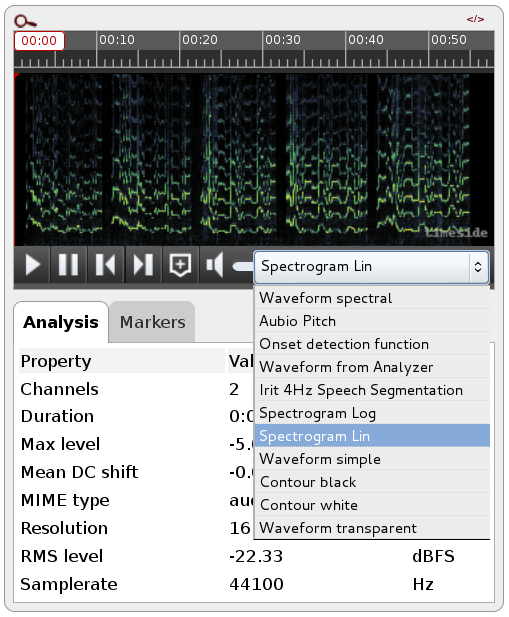
\includegraphics[width=0.9\linewidth]{img/sound_representation.png}
  \caption{Selection of various \\sound representations}
  \label{fig:sound_representation}
\end{subfigure}
\caption{Telemeta web interface}
 \end{figure*}
The flexible and streaming safe architecture is represented in Figure~\ref{fig:TM_arch}.
\begin{figure}[htb]
  \centering
  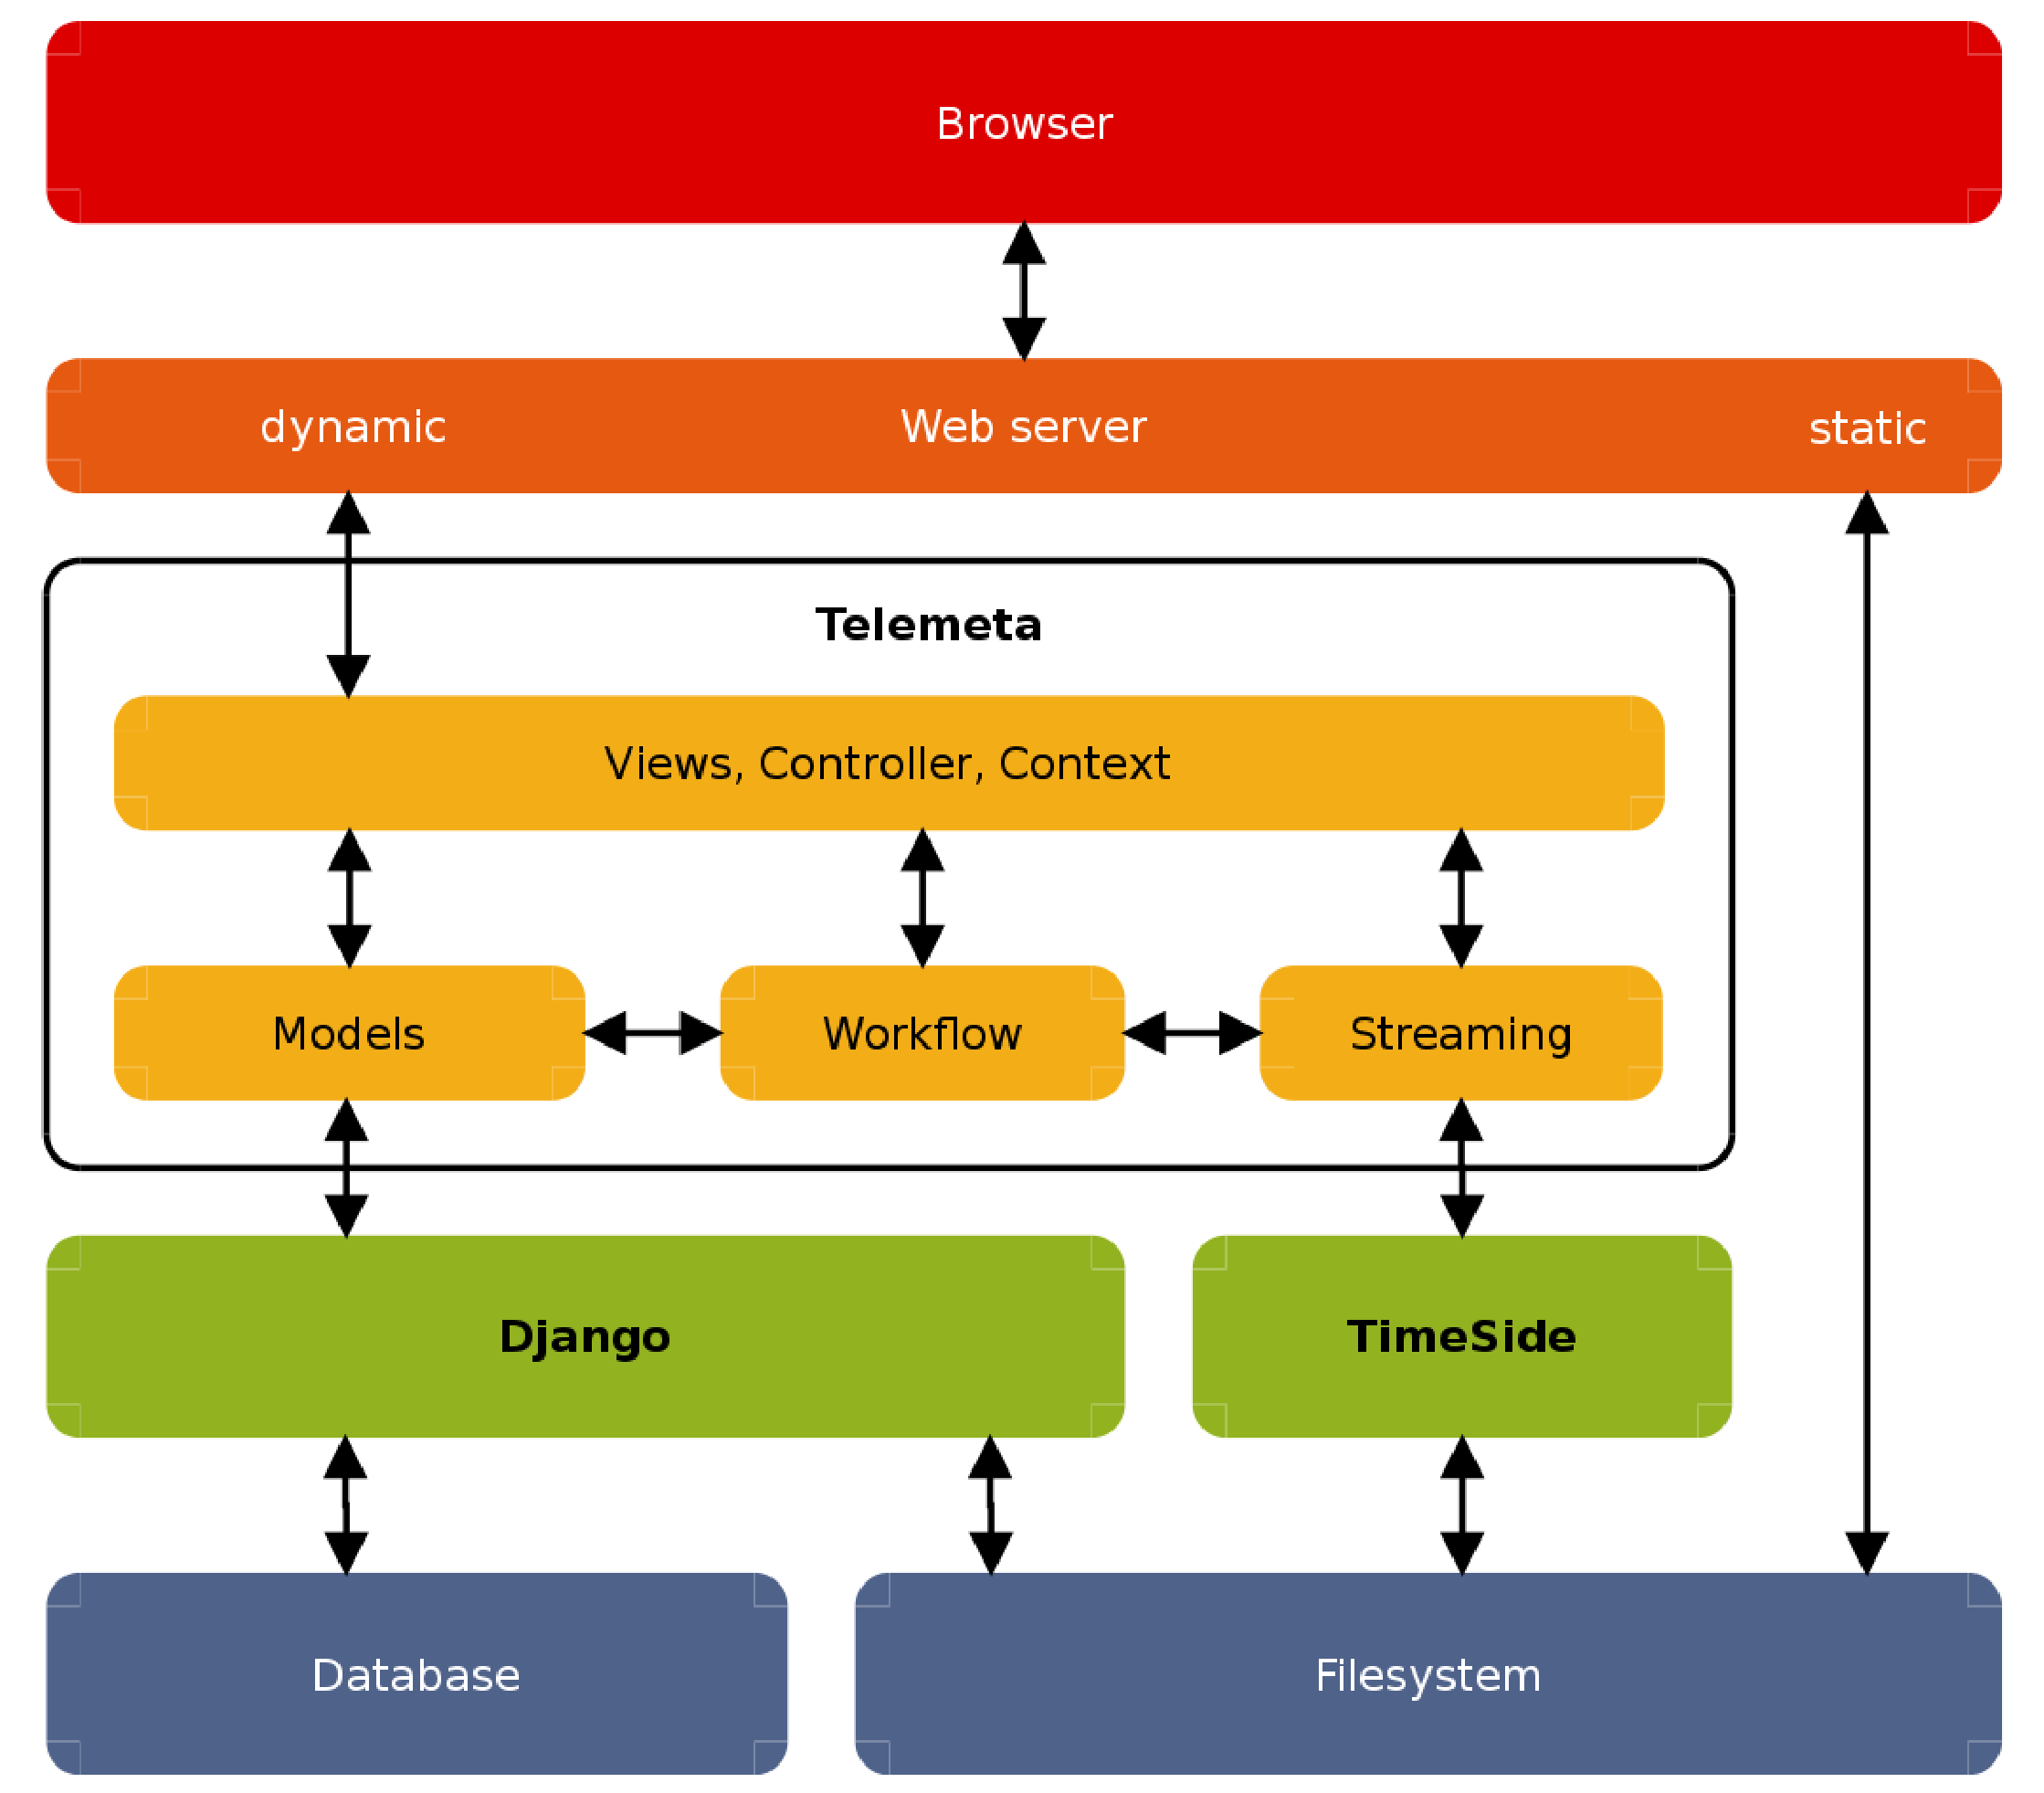
\includegraphics[width=0.9\linewidth]{img/TM_arch.pdf}
  \caption{Telemeta architecture}\label{fig:TM_arch}
  \label{fig:screenshot}
\end{figure}
The main features of Telemeta are:
      \begin{itemize}
      \item Pure HTML5 web user interface including dynamic forms.
      \item On-the-fly audio analyzing, transcoding and metadata.
        embedding in various multimedia formats.
      \item Social editing with semantic ontologies, smart workflows,
        realtime tools, human or automatic annotations and
        segmentations.
      \item User management with individual desk, playlists, profiles
        and group access rights.
      \item High level search engine (geolocation, instruments, ethnic groups, etc...).
      \item Data providers : DublinCore, OAI-PMH, RSS, XML, JSON and other.
      \item Multi-language support (currently english and french).
      \end{itemize}
Beside database management, the audio support is mainly provided through an external component, TimeSide, which is described in Section~\ref{sec:TimeSide}.
\subsection{Metadata}\label{sec:metadata}
In addition to the audio data, an efficient and dynamic management of the associated metadata is also necessary. Metadata provides valuable information about the source of the data and to the related work of peer researchers. 
Dynamically handling metadata in a collaborative manner optimizes the continuous process of knowledge gathering and the enrichment of the materials in the database.  
One of the major challenges is the standardization of audio and metadata formats with the aim of long-term preservation and usage of the different materials.
The compatibility with other systems is facilitated by the integration of the metadata standards protocols Dublin Core\footnote{{Dublin Core} Metadata Initiative, \url{http://dublincore.org/}} and \emph{OAI-PMH} (Open Archives Initiative Protocol for Metadata Harvesting)\footnote{\url{http://www.openarchives.org/pmh/}}.
The metadata includes two different kinds of information about the audio item: contextual information and analytical information of the audio content.
\subsubsection{Contextual Information}
In an ethnomusicological framework, contextual information may include details about the location where the recording was made, the instruments, the population, the title of the musical piece, the cultural elements related to the musical item, the depositor, the collector, the year of the recording and the year of publication of papers describing the work. 
Moreover, through the platform, diverse materials related to the archives can be stored, such as iconographies (digitalized pictures, scans of booklets and field notes, and so on), hyperlinks and biographical information about the collector. 

\subsubsection{Descriptive and analytical information on the audio content}
The second type of metadata consists of information about the audio content itself. This metadata can provide information about the global content of the audio item or provide temporally-indexed information. It should also be noted that such information can be produced either by a human expert or by an automatic computational audio analysis (see Section~\ref{sec:TimeSide} below).

\squeezeup\paragraph{Visual representation and segmentation}
As illustrated in Figure~\ref{fig:sound_representation}, the TimeSide audio player embedded in the Telemeta web page view of a sound item allows for a selection of various visual representations of the sound (e.g. waveforms and spectrograms, see section~\ref{sec:TimeSide} for details) and some representations of computational analysis.

Automatic analysis can produce a list of time-segments associated with labels.
Those labels have been specified by the partners of the DIADEMS project to be relevant for ethnomusicological studies (e.g. detection of spoken versus singing voices, chorus, musical instrument categories, and so on, see Section~\ref{sec:Diadems}).

\squeezeup\paragraph{Annotations}
As illustrated in Figure~\ref{fig:Telemeta}, the embedded audio player also enables annotation of the audio content through time-coded markers.
Such annotations consist of a title and a free text field associated with a given time position.

Ethnomusicologists, archivists, anthropologists, linguists and acousticians working on sound documents can create their own annotations and share them with colleagues. These annotations are accessible from the sound archive item web page and are indexed through the database.

The possibility for experts to annotate time-segments over a zoomable representation of the sound is currently under development in order to improve the accuracy and the quality of time-segment-based annotations.


\section{TimeSide, an audio analysis framework}\label{sec:TimeSide}
As illustrated in Figure~\ref{fig:TM_arch}, the Telemeta architecture relies on an external component, TimeSide\footnote{\url{https://github.com/yomguy/TimeSide}}, that offers audio player web integration together with audio signal processing analysis capabilities. 
TimeSide is an audio analysis and visualization framework based on both Python and JavaScript languages that provides state-of-the-art signal processing and machine learning algorithms together with web audio capabilities for displaying and streaming files.
Figure~\ref{fig:TimeSide_Archi} illustrates the overall architecture of TimeSide together with the data flow between TimeSide and the Telemeta web-server.
\begin{figure}[htbp]
  \centering
  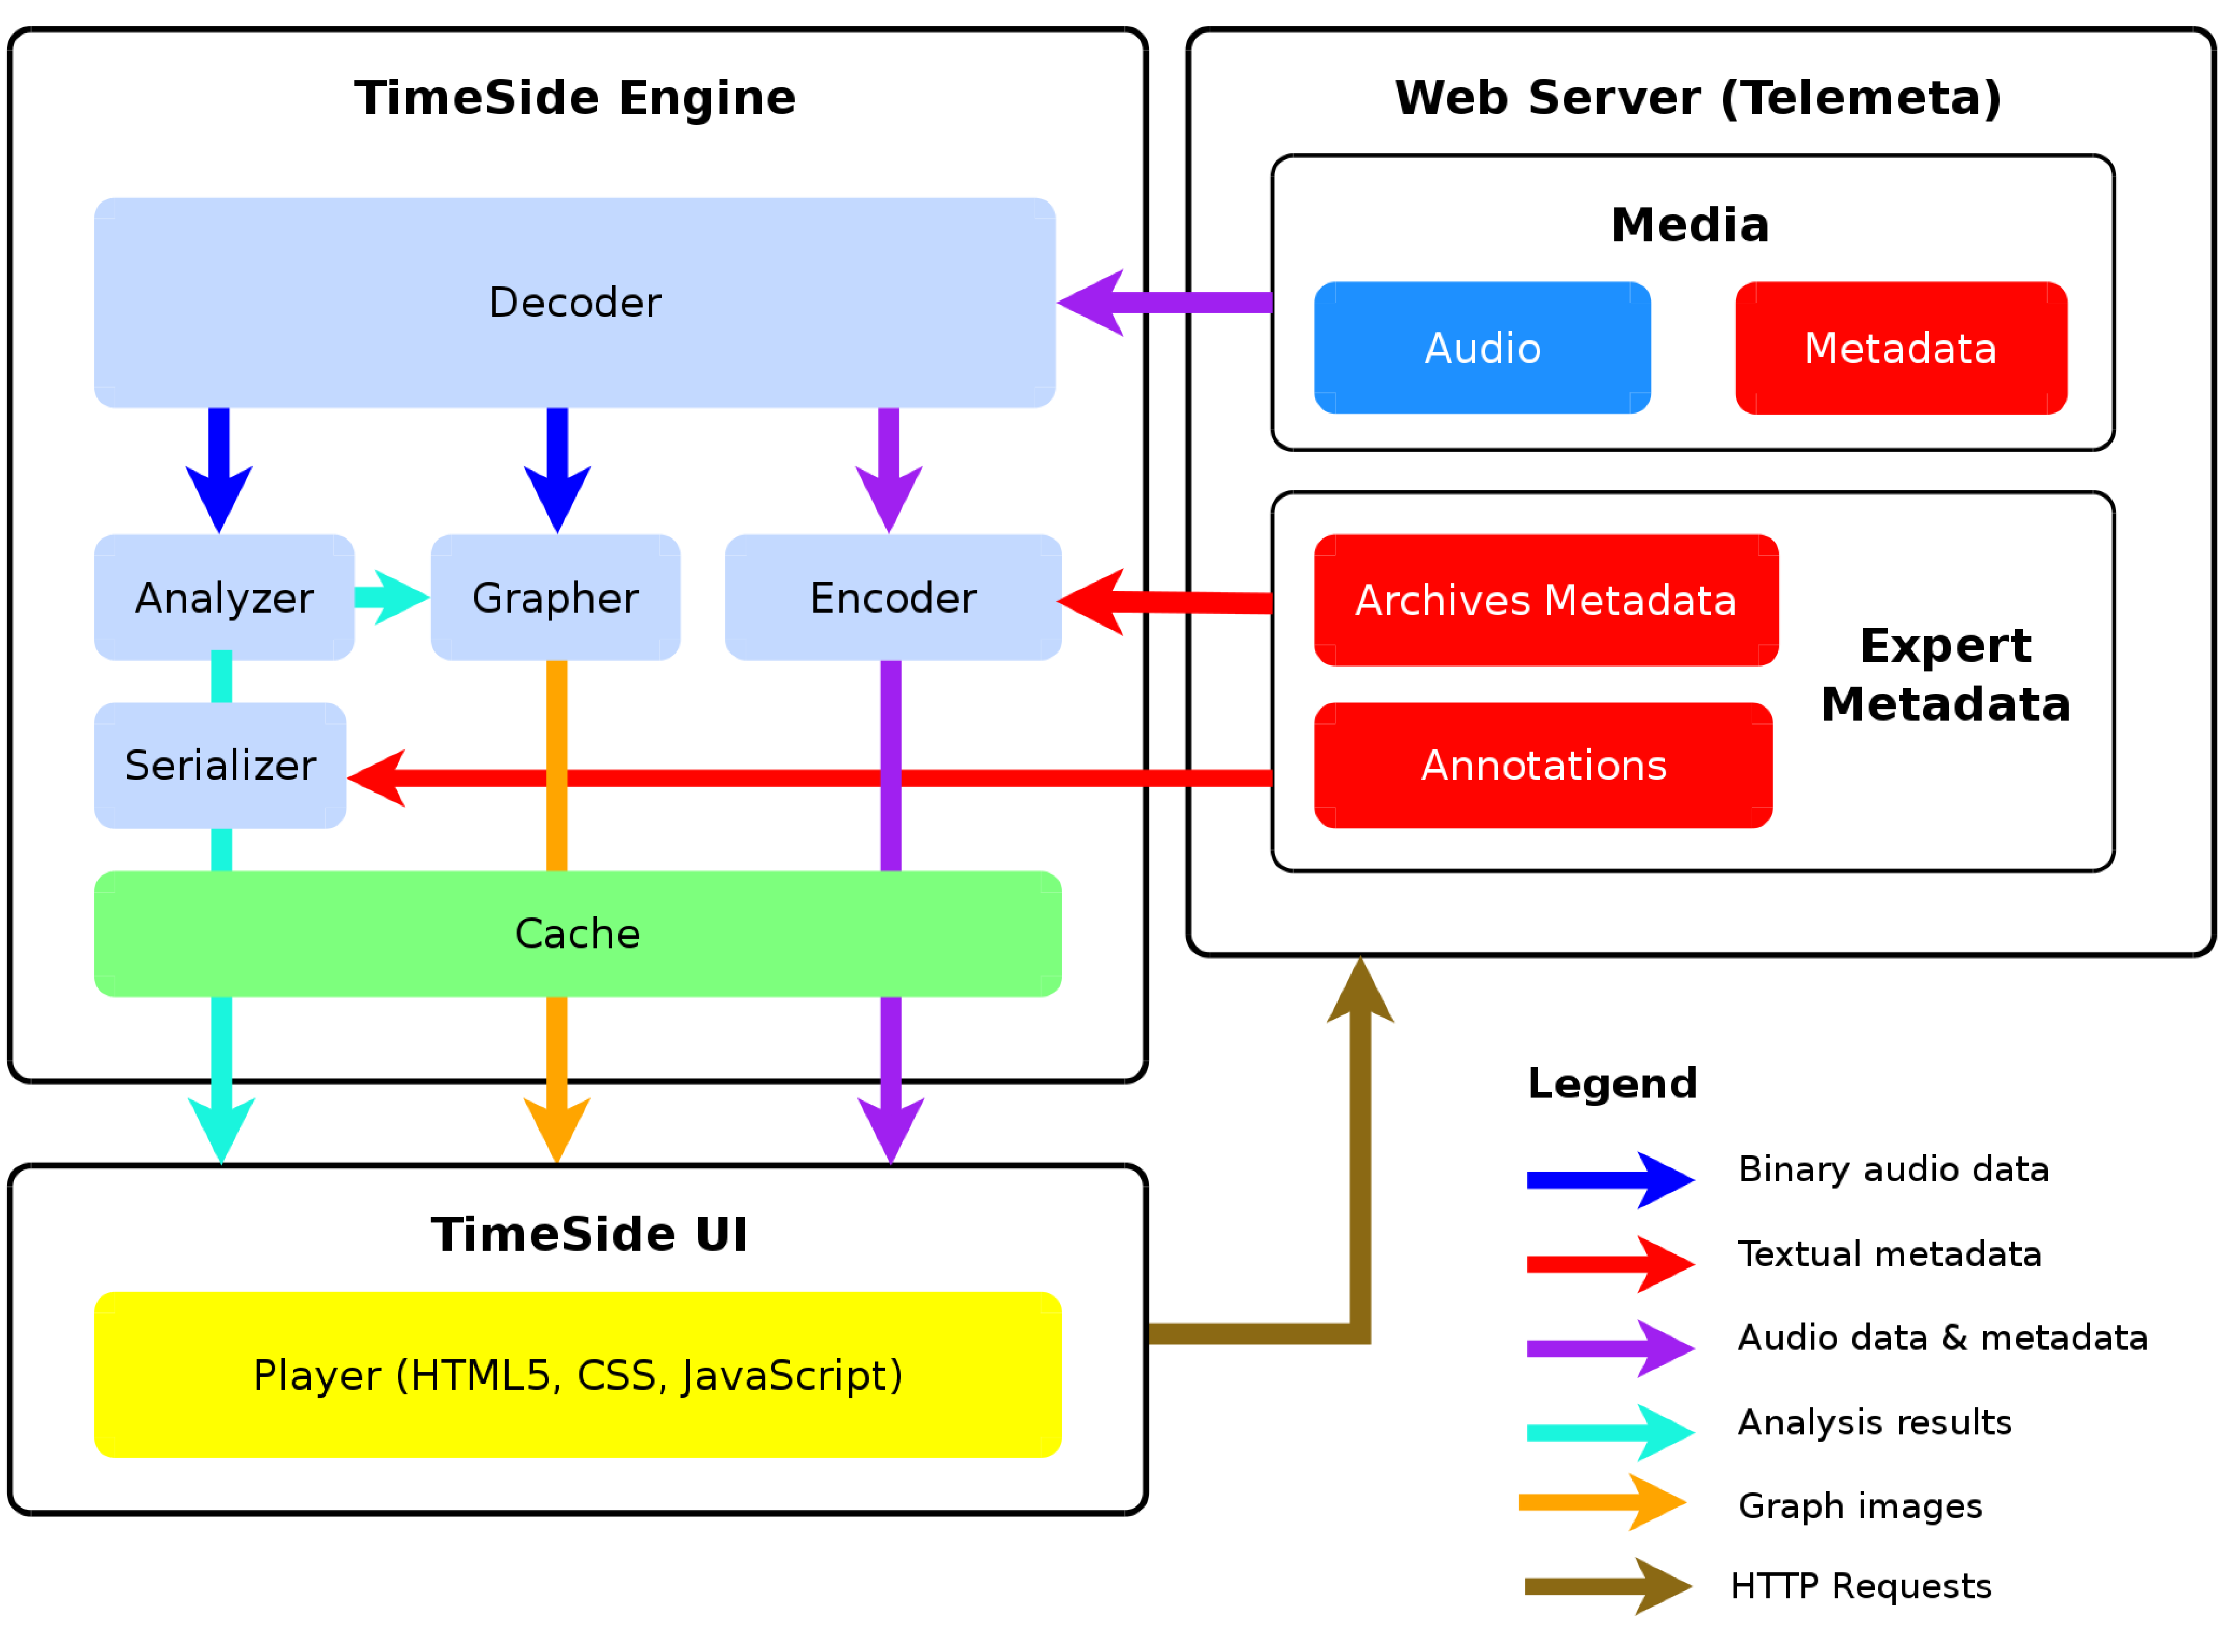
\includegraphics[width=\linewidth]{img/timeside_schema_v3.pdf}
  \caption{TimeSide engine architecture and data flow with Telemeta web-server}\label{fig:TimeSide_Archi}
\end{figure}

\subsection{Audio management}
TimeSide provides the following main features:
\begin{itemize}
\item Secure archiving, editing and publishing of audio files over
  the internet.
\item Smart audio player with enhanced visualization (waveform, spectrogram).
\item Multi-format support: decodes the vast majority of audio and video formats through Gstreamer and transcodes them with smart streaming and caching methods.
\item On-the-fly audio analysis, transcoding and metadata embedding based on an easy plugin architecture.
\end{itemize}
\subsection{Audio features extraction}
In order to implement Music Information Retrieval (MIR) analysis methods for large corpora for ethnomusicological studies, TimeSide incorporates some state-of-the-art audio feature extraction libraries such as Aubio\footnote{\url{http://aubio.org/}} \cite{brossierPhD}, Yaafe\footnote{\url{https://github.com/Yaafe/Yaafe}} \cite{yaafe_ISMIR2010} and Vamp plugins\footnote{ \url{http://www.vamp-plugins.org}}.
Given the extracted features, every sound item in a given collection can be automatically analyzed. The results of this analysis can be stored in a scientific file format (e.g. NumPy format and HDF5), exported to sound visualization and annotation software like sonic visualizer \cite{cannam2006sonic}, or serialized to the web browser through common markup languages: XML, JSON and YAML.

Telemeta's open-source framework and architecture, combined with the flexibility provided by Python, facilitates the implementation of many audio and music analysis algorithms and their application to audio archives. Thus, Telemeta is an interesting platform for researchers in computational musicology who wish to develop and evaluate their algorithms.


\section{Sound archives of the \\CNRS - Musée de l'Homme}\label{sec:archives-CREM}
Since June 2011, the Telemeta platform has been used by the  Sound archives of the CNRS - Musée de l'Homme\footnote{\url{http://archives.crem-cnrs.fr}} and managed by the CREM. According to the CREM specific aims, the Telemeta platform makes these archives available for researchers, students and (when copyright allows) to a broader audience. Through this platform, these archives can be shared, discussed and analyzed.

The Telemeta platform has also been deployed for the sound archives of the \emph{Laboratory of Musical Acoustic} of the ``Jean Le Rond d'Alembert Institute''\footnote{\url{http://telemeta.lam-ida.upmc.fr/}. Online since 2012, these archives consist in recordings of a wide range of musical instruments, mostly including solo recording of traditional instruments and illustrating various playing techniques and are used as materials for research in acoustics.}.



\subsection{Archiving research materials}
The Sound archives of the CNRS - Musée de l'Homme is one of the most important in Europe and contains commercial and unpublished recordings of music and oral traditions from around the world, collected by researchers attached to numerous research institutions across the world, including prominent figures of the field of ethnomusicology (among which Brailoiu, Lomax, Shaeffner, Rouget and Elkin). 

The platform offers access to record collections (nearly 3700 hours, e.g. more than 5000 discs, many of which are very rare) and to 4000 hours of unpublished recordings, from early research expeditions (e.g. Dakar-Djibouti (1932), Ogooué-Congo (1946)). Most of the recordings come from the fieldwork of researchers in all continents. 
More than 110 years of the world's oral culture are now available online, from the 1900 Universal Exhibition of Paris to recent digital recordings. The sharing of data allows several people to collaborate on the enrichment of the database. Today, 47,200 items are in the database, and more than 26,000 sound files have been included (12,000 sounds on free access since May 2014). Recently, the CREM has decided to give full access to the records published by the CNRS-Musée de l’Homme (Chant du Monde/Harmonia Mundi)\footnote{\url{http://archives.crem-cnrs.fr/archives/fonds/CNRSMH_Editions/}}, the distribution of which stopped ten years ago.
As a web platform, this tool is also a way to cross borders, to get local populations involved in their own cultural heritage and to offer resources to researchers from all over the world.

\subsection{Uses and users of digital sound archives}
In the few years since the sound archive platform has been released, it has supported three main activities: archiving, research and education (both academic and non-academic). Primary users of the platform are archivists, researchers (ethnomusicologists, anthropologists and linguists), students and professors of these disciplines. Nonetheless, a qualitative survey showed that other disciplines (such as art history) have used the platform to foster and/or deepen individual research. The unexpectedly broad uses of the sound archives emphasize the necessity and the benefits of such database.
From the standpoint of archive development, the long-term preservation of the archives is ensured while, thanks to the collaborative nature of the platform, users can cooperate to continuously enrich metadata associated with a sound document and submit their own archives to protect them. Furthermore, it facilitates the ethical task of returning the recorded music to the communities who produced it.
Researchers from different institutions can work together on specific audio materials and conduct individual research from both synchronic and diachronic perspectives on their own material, the material of others, or both.
When used for education, the platform provides a wide array of teaching materials to illustrate the work of students as well as support teaching curricula.



\section{Expanding development: the DIADEMS project}\label{sec:Diadems}

The many goals and expectations of the platform expand through time, as users experience new ways to work with the archives and request new tools to broaden the scope of their research activities linked to it. Comments from engineers and researchers on their usage of the sound archives database led us to set up a large scale project called DIADEMS (\emph{Description, Indexation, Access to Ethnomusicological and Sound Documents})\footnote{\url{http://www.irit.fr/recherches/SAMOVA/DIADEMS/en/welcome/}}. 
%DIADEMS is a French national research program, started in January 2013, with three IT research labs (IRIT\footnote{Institut de Recherche en Informatique de Toulouse}, , , LIMSI\footnote{Laboratoire d’Informatique pour la Mécanique et les Sciences de l’Ingénieur}, LABRI\footnote{Laboratoire Bordelais de Recherche en Informatique})\comment{TF: + LAM + labo ethno + Parisson. Plutôt dire a collaboration between ethno + IT}
Started in January 2013, the French national research program DIADEMS is a multi-disciplinary project whose consortium includes research laboratories from the \emph{ Science and Technology of Information and Communication}\footnote{IRIT (Institute of research in computing science of Toulouse), LABRI (Bordeaux Computer Science Research Laboratory), LIMSI (Laboratory of computing and mechanics for engineering sciences), LAM (Laboratory of Musical Acoustic, Jean Le Rond d'Alembert Institute)} (IT) domain, the \emph{Musicology and Ethnomusicology}\footnote{LESC (Laboratory of Ethnology and Comparative Sociology), MNHN (National Museum of Natural History)} domain and Parisson, a company involved in the development of Telemeta.
 
The goal of the DIADEMS project is to develop computer tools to automatically index the recording content directly from the audio signal in order to improve access to and indexation of this vast ethnomusicological archive. Numerous ethnomusicological recordings contain speech and other types of sound that we categorized as sounds from the environment (such as rain, biological sounds, engine noise and so on) and sounds generated by the recording process (such as sound produced by the wind on the microphone or sounds resulting from defects of the recording medium). The innovation of this project is to automatize the indexation of the audio recordings directly from the recorded sound itself. Ongoing work consists of implementing advanced classification, indexation, segmentation and similarity analysis methods dedicated to ethnomusicological sound archives.  Besides music analysis, such automatic tools also deal with speech and other types of sounds classification and segmentation to enable a more exhaustive annotation of the audio materials.

%The goal of Diadems project is to propose a set of tools for automatic analysis of audio documents which may contain fields recordings: speech, singing voice, instrumental music, technical noises, natural sounds, etc. The innovation is to automatize the indexation of  audio recordings directly from the audio signal itself, in order to improve the access and indexation of anthropological archives. Ongoing works consist in implementing advanced classification, segmentation and similarity analysis methods,  specially suitable to ethnomusicological sound archives. The aim is also to propose tools to analyse musical components and musical structure. 
The automatic analysis of ethnomusicological sound archives is considered to be a challenging task.
Field recordings generally contain more sound sources, noise, and recording artefacts than those obtained in studio conditions, so the automatic analysis of these recordings requires robust methods.
Preliminary implementations  of speech detection models and speaker diarization methods based on \cite{barras2006multistage} have been integrated to TimeSide. 
While these models are well suited to radio-news recordings, the current development task is to adapt them to the particular case of ethnographic archives.

In the context of this project, researchers from the Ethnomusicological, Speech Processing and MIR communities are working together to specify the tasks to be addressed by automatic analysis tools.


\subsection{The method of a new interdisciplinary research}

In this research program, groups from different backgrounds are working together to specify the automatic analysis tools. Participants include IT developers, humanities researchers (anthropologists, ethnomusicologists, ethnolinguists) and specialists in speech processing and MIR. The first challenge was to initiate a common interest and a mutual understanding. In this process, DIADEMS gave us the opportunity  to improve our understanding on the link between the semantics and acoustics of voice production. 
In preliminary work, we attempted to first define vocal categories with a particular interest for liminal oral productions. At the border between speech and song, utterances such as psalmody or recitation are at the center of an old debate in ethnomusicology\footnote{A colloquium on liminal utterances between speech and song will be organized by the International Council for Traditional Music (ICTM) in May 2015 and hosted by the Centre of research in Ethnomusicology (CREM). A round table will be dedicated to the presentation of the main results and findings of the ANR project DIADEMS}. Gathering specialists from various fields, the DIADEMS project goes well beyond the usual disciplinary boundaries. Our aim, through the study of a large range of audio components (pitch range, syllabic flow, metric, polyphonic and so on) is to define and characterize the variability of vocal productions, keeping in mind the semantic aspects. By doing so, we wish to reduce the traditional gap in academic studies between sounds and semantics and to develop combined analytical tools for the study of vocal production\footnote{As an example, research will be conducted on the recognition of "icons of crying" 
in lamented utterances. As defined by Urban in \cite{Urban88}, "icons of crying" include cry break, voice inhalation, creaky voice and falsetto vowels.}. 

One of the goals of the DIADEMS project is also to provide useful tools for musical analysis such as the detection of musical instrument families, analysis of musical content (tonal, metric and rhythmic features), musical similarities and structure (chorus localisation, musical pattern replication).

The study follows three steps : 
\begin{enumerate}
\item The development of tools and selection of a representative corpus
  for each tool.
\item The evaluation of the proposed automatic analysis, in addition to
  the human-led evaluations carried out on the selected corpus.
\item The development of a visual interface for accessing and contributing to the database.
\end{enumerate}



\subsection{Automatic tools for assisting indexation and annotation of audio documents}
A first concern was to develop an automated annotation component that could differentiate spoken from sung voice and from instrumental music. State-of-the-art methods for this tasks have usually been designed to fit the needs of radio broadcast data (i.e. clear recordings produced in studios) and are not adapted to the sonic diversity of ethnomusicological field recordings. For these, more refined detection tools are needed to pick up sound events such as overlapping speech from multiple speakers, speech over music, and instrumental music mixed with singing and/or spoken interventions.
Beyond the implementation of tools for detecting the beginning and end of sound signatures of magnetic, mechanical and digital recorders as well as tape noises and silences, the platform provides algorithms for the complex automated analysis of a wide range of combinations of vocal and instrumental sounds.


\subsubsection{Analysis of recording sessions}
A primary concern of people dealing with field recordings is the fast and accurate identification of the start and the stop times of a recording session.

In the case of digital recorders, the proposed system for localizing the start of recording sessions is based on the observation that on such recorders, the powering of the recorder implies a characteristic and quite reproducible perturbation of the signal as illustrated in Figure~\ref{plop}. Therefore, this perturbation can be modeled by using some reference models of the shape of the temporal energy. On the analyzed recordings, the evolution of the temporal energy of low energy segments is then compared to the models by a euclidean distance using the best alignment of the energy shape.

\begin{figure}[htb]
 \centering
    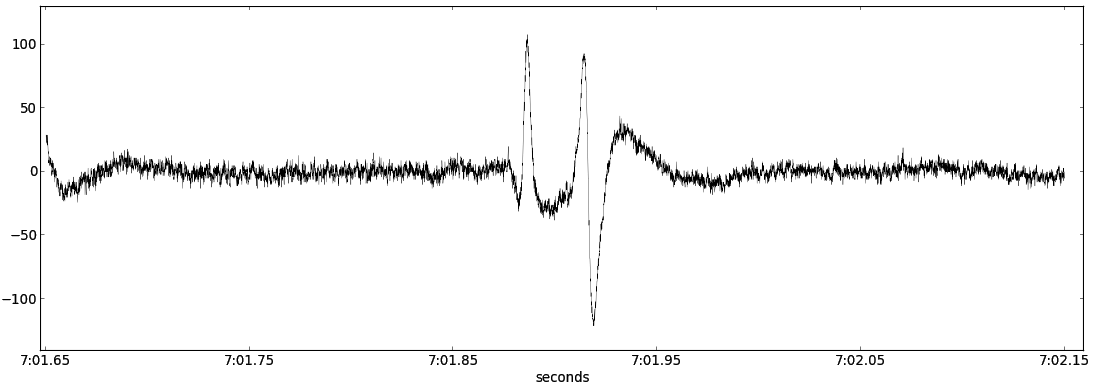
\includegraphics[width=0.8\linewidth]{img/plop.png}
    \caption{Typical perturbation produced by the recorder powering-on, used to recognize the start time of a session.}
    \label{plop}
\end{figure}


\subsubsection{Analysis of speech and singing voice segments}
The quick identification and localization of spoken sections, particularly in rather long recordings, is important for all the disciplines involved in this project. Difficulties inherent in the processing of sound materials led to the development of tools to automatically detect occurrences of speech when performed simultaneously with music. The detection of speech is important in a number of scenarios, such as when numerous speakers interact and/or overlap with each others---with or without additional music or noises---and when voices modulate from speech to song, using a wide range of vocal techniques (recitation, narration, psalmody, back channel, and so on). The developed algorithms allow the analysis of the syllabic flow and the prosody of the speech. 
Figure~\ref{fig:speech_detection} shows a visual example of how speech segmentation is rendered.

%Source : CNRSMH_I_2013_201_001_01/
\begin{figure}[htb]
  \centering
 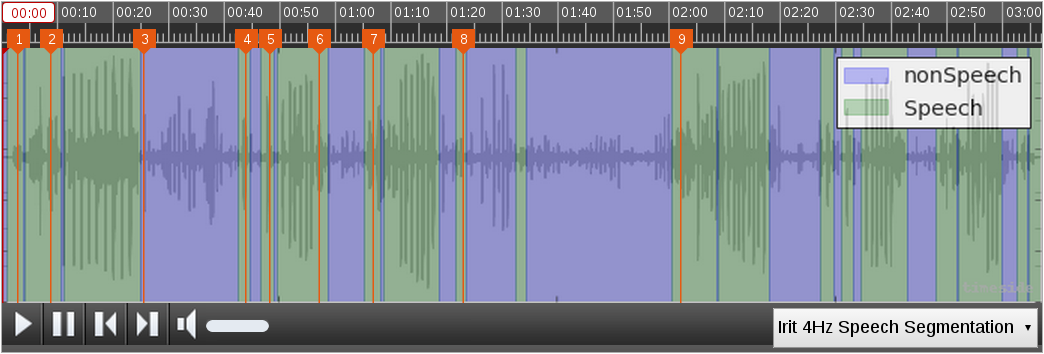
\includegraphics[width=\linewidth]{img/IRIT_Speech4Hz.png} 
  \caption{Detection of spoken voices in a song}
  \label{fig:speech_detection}
\end{figure}

\squeezeup\paragraph{Speech segmentation with 2 features: 4 Hz modulation energy and entropy modulation} 
Speech signal has a characteristic energy modulation peak around the 4 Hertz syllabic rate \cite{Houtgast1985}. In order to model this property, the signal is filtered with a FIR band pass filter, centered on 4 Hertz.
Entropy modulation is dedicated to discriminate between speech and music~\cite{Pinquier2003}. We first evaluate the signal entropy ($H=-\sum_{i=1}^{k}p_i\cdot \log_2(p_i)$, where $p_i$ denotes the probability of event~$i$). Entropy modulation values are usually larger for speech than for music. This measure is used to compute the entropy modulation on each segment. 

\squeezeup\paragraph{Speech activity detection based on GMM models}
Speech activity detection is a prerequisite for several speech-related tasks to be integrated in the platform such as speech segmentation, speaker diarization and so on.
For this approach, a Gaussian Mixture Model system operating at the frame level, is used to learn speech spectral properties from annotated data.
MFCC, together with their first and second time derivative, log energy and zero crossing rate audio features are used to train the GMM models to discriminate speech frames from non speech frames.
The ETAPE corpus \cite{gravier2012etape} (speech-based TV archives in French), and data obtained from the French Center of Research and Teaching on Amerindian Ethnology (carnival rituals in Mayan language) were used to train two distinct sets of models.
Both models have been serialized and integrated into TimeSide together with the GMM-based speech activity detection system, allowing the final user to choose a given model according to the properties of the media to analyze.

\subsubsection{Analysis of music segments}
The DIADEMS project aims to provide useful tools for musical analysis in both research and teaching frameworks. Thus, the detection of segments of instrumental music along with the recognition of the different musical instrument categories is needed. The implemented tools provide musicological information to support sound analysis (such as tonal, metric and rhythmic features) and to allow the detection of similarities in melody, harmony and rhythm, as well as musical pattern replications.

\squeezeup\paragraph{Music segmentation with 2 features based on a segmentation algorithm} 
This segmentation is provided by the Forward-Backward Divergence algorithm, which is based on a statistical study of the acoustic signal \cite{Obrecht1988}. The speech signal is assumed to be composed of a sequence of quasi-stationary units that can be seen as alternate periods of transient and steady parts (steady parts are mainly vowels). We characterize  each of these units by an Auto Regressive (AR) Gaussian model. The method detects changes in AR models. Indeed, music is usually much more constant than speech, that is to say the number of changes (segments) will be smaller for music than for speech. To estimate this, we count the number of segments per second of signal. The number of segments is the first discriminative feature for music segmentation.
The segmentation algorithm  generally produces longer segments for music than for speech. We chose to model the segment duration by an inverse Gaussian distribution (or Wald distribution) which is indeed the second feature providing music segmentation.


\squeezeup\paragraph{Monophony / Polyphony segmentation}
A ``monophonic'' sound is defined as one note played at a time (either played by an instrument or sung by a singer), while a ``polyphonic'' sound is defined as several notes played simultaneously. The parameters extracted from the signal come from the YIN algorithm, a well known pitch estimator \cite{DeCheveigne2002}. Besides F0, this estimator provides an additional numerical value that can be interpreted as the inverse of a confidence indicator (the lower the value, the more reliable the estimated pitch). 
Considering that the estimated pitch is fairly accurate when there is a single note, and that the estimated pitch is not reliable when there are several simultaneous notes, we take the short term mean and variance of this ``confidence indicator'' as parameters for the monophony / polyphony segmentation. The bivariate distribution of these two parameters is modelled using Weibull bivariate distributions \cite{Lachambre2011}.
An example of the segmentation produced by this method is illustrated in Figure~\ref{fig:Monopoly}
% Source : CNRSMH_I_2000_008_001_04
\begin{figure}[htb]
  \centering
%\framebox[1.1\width]{Capture d'écran de IRIT Monopoly}
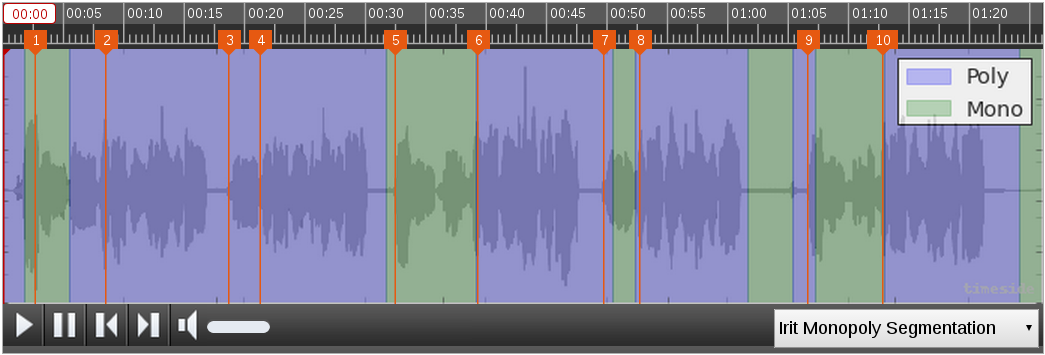
\includegraphics[width=0.95\linewidth]{img/SOLO_DUOdetection.png} 
 \caption{Detection solo and duo parts}
  \label{fig:Monopoly}
\end{figure}

\squeezeup\paragraph{Automatic instrument classification}
For the detection of musical instruments, we choose to follow the Hornbostel–Sachs system of musical instrument classification as first published in \cite{taxonomy_sachs2} and later translated in \cite{taxonomy_sachs}. This system is the most widely used system for classifying musical instruments by ethnomusicologists and organologists. It was extended by in more recent systems like the one proposed by Geneviève Dournon in \cite{Dournon92} and the \emph{RAMEAU} reference from the French national library (BnF)\footnote{\url{http://catalogue.bnf.fr/ark:/12148/cb119367821/PUBLIC}}.

We choose to develop tools to detect the four musical instrument families (cordophones, aerophones, idiophones, membranophones), but also to refine subdivisions related to the playing techniques, identifying whether each instrument is blown, bowed, plucked, struck or clincked by focusing on the 8 classes of instrument shown in Figure~\ref{fig:instruments}.

\begin{figure}[htb]
  \centering
  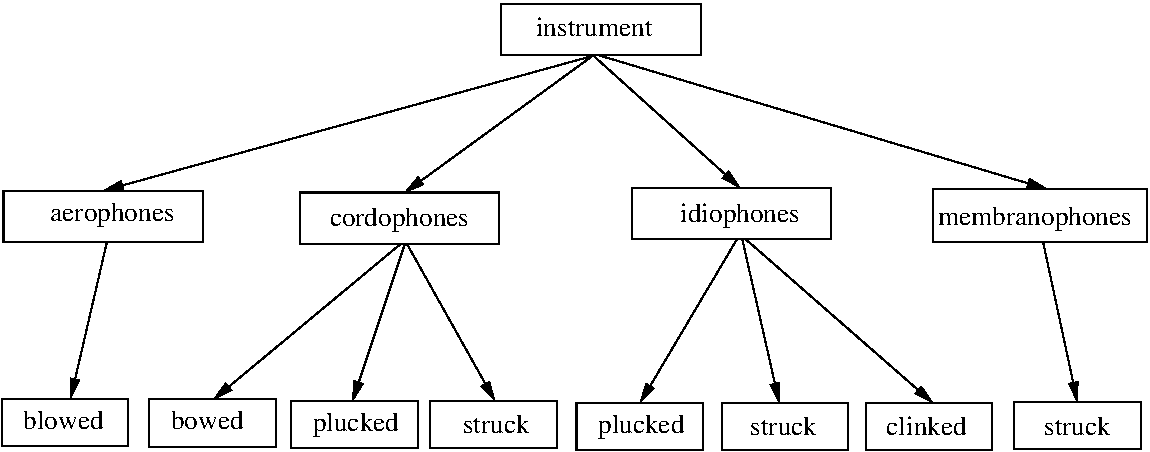
\includegraphics[width=0.9\linewidth]{img/taxonomie_diadems.pdf}
  \caption{Musical instrument families}
  \label{fig:instruments}
\end{figure}

The proposed method is based on the supervised learning approach and uses a set of 164 acoustic descriptors 
proposed by Peeters \textit{et al.} in \cite{timbre_toolbox}.
This system (see Figure~\ref{fig:inst_classif_method}) applies the Inertia Ratio Maximization Features Space (IRMFSP) algorithm~\cite{aes_irmfsp} 
on annotated samples at the training step to reduce the number of features (to avoid overfitting) while selecting the most discriminative ones. %% see Figure 6

\begin{figure}[htb]
 \centering
 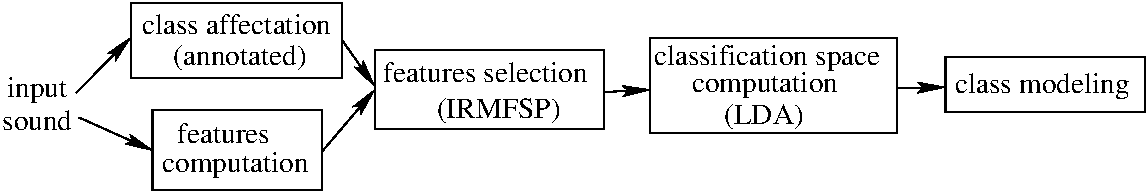
\includegraphics[width=0.9\linewidth]{img/method}
 \caption{Training step of the proposed classification method}
 \label{fig:inst_classif_method}
\end{figure}

The Linear Discriminant Analysis (LDA) method~\cite{lda_book} is used to compute the best projection space 
or linear combination of all descriptors which maximizes the average distance between classes while minimizing the 
distance between individuals of the same class.

Each class is simply modeled in the classification space by its centroid (mean vector computed over the selected descriptors of the individuals which compose the class).
Thus, the classification task consists of projecting each tested sound described by a vector of descriptors
into the classification space and selecting the closer class (in term of Euclidean distance to the class centroid). 

This simple and computationally efficient method reaches an accuracy of 75\% 
using the 20 most relevant descriptors projected on an 8-dimensional discriminative space. In a more detailed study~\cite{ismir14_dfourer},
this promising result was shown to be comparable with state-of-the art methods applied to the classification of western instruments recorded in studio conditions.

% \begin{figure}[!ht]
%  \centering
% 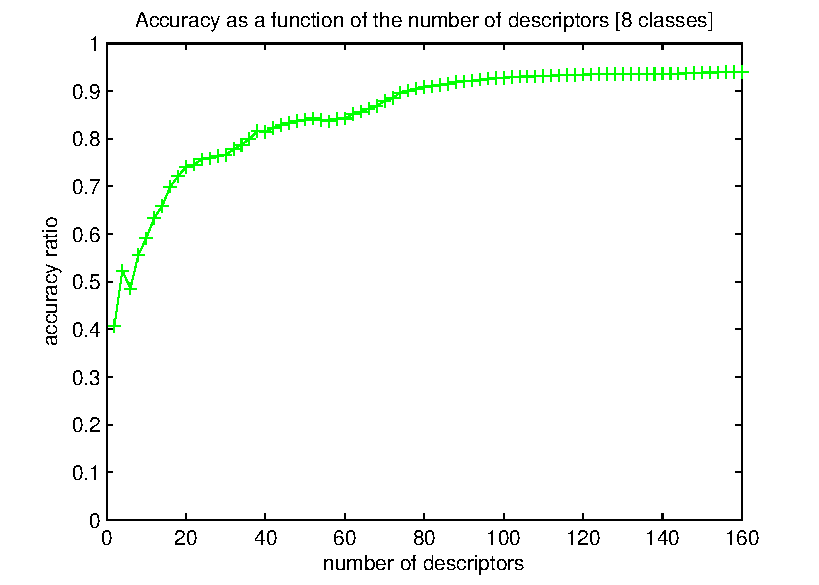
\includegraphics[width=0.7\linewidth]{img/crem_results}
%  \caption{3-fold cross-validation classification accuracy as a function of the number of optimally selected descriptors.}
%  \label{fig:inst_classif_result}
% \end{figure}


\subsection{Evaluation and future improvements}

At the end of the first step of the project, interesting preliminary results have been obtained regarding the detection of start times of recording sessions, speech recognition, singing voice recognition and musical instrument family classification.

Through collaborative work, ethnomusicologists, ethnolinguists and engineers are currently evaluating, correcting and refining the implemented tools, with the expectation that these new tools will be integrated into the Telemeta platform. 

The robustness of these processing is assessed using criteria defined by the final users: teachers, students, researchers and musicians. Annotation tools, as well as the provided annotations, will be integrated in the digitalized database. 

Further work on the user interface will enhance the visualization experience with time and frequency zooming capabilities, in the hope that it will improve the accuracy and the quality of time-segment based annotation. One of the remaining goals is to develop tools to generate results online and to make use of the capabilities of Internet browsers while managing the workflow. 


\section{Conclusion}
 The Telemeta open-source framework provides a new platform for researchers in humanities and social sciences to efficiently distribute, share and work on their research on musical and sound materials. 
This platform offers automatic music analysis capabilities through the external component, TimeSide, which provides a flexible computational analysis engine together with web serialization and visualization options. 
The Telemeta platform provides an appropriate processing framework for researchers in computational ethnomusicology to develop and evaluate their algorithms. 
Deployed to manage the CNRS - Musée de l’Homme sound archives, the Telemeta platform has been conceived and adapted to generate tools in line with the needs of users. 

Thanks to the collaborative nature of the platform, users can continuously enrich metadata associated with sound archives. 
The benefits of this collaborative platform for the field of ethnomusicology apply to numerous aspects of research, ranging from musical analysis in diachronic and synchronic comparative perspectives, as well as the long-term preservation of sound archives and the support of teaching materials for education. 


\section{Acknowledgments}
The authors would like to thank all the people who have been involved in Telemeta specification and development or who have provided useful input and feedback. 
The project has been partly funded by the French National Centre for Scientific Research (CNRS), the French Ministry of Culture and Communication, the TGE Adonis Consortium, and the CREM.


\bibliographystyle{abbrv}
\bibliography{dlfm2014_Telemeta}

%\listofchanges

\end{document}
 
 
